

One of the challenges in brain research is finding relationships between the physical structure of the brain and the way it functions. Structural information is gathered mainly through the use of imaging techniques as Magnetic Resonance Imaging (MRI), Computer Aided Tomography (CAT) or Positron Emission Tomography (PET). Other methods measure the electrical activity of the brain, as in Electro-Encephalography  (EEG) or Magneto-Encephalography (MEG). Transcranial Magnetic Stimulation (TMS) is a technique where cells are stimulated using a rapid changing magnetic field, which in turn generates an electrical field inside the neurons, the effects of this stimulation are measured elsewhere.

Traditionally research is done by formulating hypotheses and designing experiments to test such hypotheses. Next, subjects are recruited, the experiment is performed on each subject and data is gathered. Finally this data is analyzed using statistical methods which provide evidence in favor or against the hypothesis. This methodology imposes limitations on how data is used. Usually data is used only once, which is unfortunate because gathering this data is expensive in time, effort and resources.

In the past several years there has been a shift towards gathering data in a more open fashion, and several public databases have appeared. There has been several improvements in the way data is collected, stored and shared, both at the technical and policy levels. Even inside small research groups, it has become more common to continue looking at the data after traditional hypothesis testing is complete.

All of this is leading to a change in the way research is done. This is a shift from hypothesis driven research into data driven research. This also creates an increased need for exploratory analysis methods, since the current ecosystem is dominated by methods created for confirmatory analysis. In this context new challenges arise. It is becoming increasingly necessary to manage, analyze and visualize data from studies in which the number of subjects is increased by orders of magnitude, as well as the measures available for each one. In this scenario it is hard to guarantee homogeneity of data for each subject. For example in large scale longitudinal studies data is typically available for each subject at several points in time.

The work-flow in this kind of analysis differs significantly from the traditional one. It requires iterating through the data several times, looking at it from different points of view, searching for relevant subjects and measures, gathering details from individuals and performing group analyzes involving several measures.

Similar scenarios have appeared in other domains, such as in economics, terrorism prevention and business intelligence. The common challenge is extracting meaningful information from large and heterogeneous data-sets. Proposed solutions often involve statistics, machine learning and databases together with efficient and intuitive interfaces and data visualizations. Visual analytics has emerged as a discipline which attempts to integrate all of these areas with the objective of making optimal use of the available data. Visual analytics recognizes the human analyst as the most important element in the task, and focuses on letting the analyst work with freedom and efficiency while focused as much as possible on the data instead of the tools.

In this thesis visual analytics techniques are applied to the particular case of cohort studies of brain data. A model which abstracts and formalizes the elements of this task is proposed. This model can be adapted and applied to other domains where cohort-like data is found. Subsequently, the model is used as the basis for the design and implementation of a software environment called BRAVIZ. This software was successfully used in a large brain study performed by the Kangaroo Foundation. This study involved analyzing data from about 450 participants. Each of them went through several neuro-psychological tests, home visits, interview, clinical evaluations and an assessment of performance in education and workforce. Additionally 250 of them went through anatomical, functional and diffusion weighted MRI.

The results are very encouraging and show that the proposed tools  helped the experts feel like they were in control of their data, could move through it freely and explore it as they liked. This provided a productive experience where information, questions and hypotheses could be gathered from the data.


\section{Visual Analytics}

%Que es

Visual analytics is a discipline which "combines automated analysis techniques with interactive
visualizations for an effective understanding, reasoning and decision making on the basis of very
large and complex datasets" \autocite{cook_illuminating_2005}. It is based on the premise that computers and
human beings have different sets of skills which should complement each other. Modern
computing systems are able to store and operate on very large amounts of data.
Specifically data-mining, clustering, machine learning and complex statistical methods can be
applied to Terabytes of data using high performance computers or clusters. These
algorithms, however, are limited in that they lack the theoretical framework, context and critical
thinking abilities necessary to make sense of data, specially when searching for the unknown.
On the other hand, domain experts have a very rich theoretical
background, expertise and intuition which allow them to grasp the meaning of data and to
make better decisions about the direction in which the analysis should move.

The goal of visual analytics is to provide an environment where humans and machines can work
together and communicate fluidly, such that the specific abilities of both are used
efficiently. Fluid communication is achieved through rich interactive
visualizations and friendly user interfaces.
The human visual system has a large capacity to process information when it is
represented in the appropriate way \autocite{ware_information_2004}. Data visualization has been studied
exhaustively in recent years and many efficient ways to represent large multidimensional
datasets have been designed \autocite{heer_tour_2010}. As
pointed by Ware: "`The best visualizations are not static images to be printed in books, but fluid,
dynamic artifacts that respond to the need for different views or for more detailed
information"' \autocite{ware_information_2004}, interactivity is a fundamental component of these systems.
However,  these interactions should be
as simple and intuitive as possible, in order to allow analysts to focus their attention on the
data itself \autocite{spence_information_2007} rather than on details of the tools.

Some visual analytics systems integrate automatic data processing algorithms with interactive data visualizations
inside a loop \autocite{keim_mastering_2010}. The goal of the loop is to extract knowledge from data. Yet again, this process
is much more efficient when automatic tools are combined with visualizations and therefore allowing the intervention of the
human expert at early stages.

The benefits of visual analytics are more evident when dealing with large and complex datasets. In this case it is also important
to have an efficient data storage infrastructure that can support all the interactive process.

Given these requirements, the design and development of effective visual analytics
applications naturally draws from diverse areas of knowledge, such as data mining, data management, perception and cognition, human-computer interaction and scientific and information visualization \autocite{keim_visual_2008}. Elements from all these areas have to be integrated smoothly in order to achieve the goal of keeping the analyst focused on the data. In many cases this means managing in the background details that are not relevant for the task at hand. The analyst is always the main character in visual analytics, and all supporting tasks must meet the analysts' needs. Therefore studying the user, including the typical workflow, and the particular analysis tasks is a requirement to design these kinds of systems.
%Ejemplos


The concepts of visual analytics'  can be applied in many domains including law enforcement, business intelligence, city planning, network analysis and bio-informatics\footnote{Tarea: Buscar referencias}. In fact the framework can be applied everywhere there is a need to extract meaning from data, specially where data is large, heterogeneus, noisy, incomplete or unstructured. However because it is centered on the domain, and particular analysis needs, a single visual analytics solution that works on every domain is not feasible. Actually the biggest contribution of visual analytics is recognizing the analyst as the most important element, and putting all these disciplines at his service in order to help him solve his analysis tasks. The analyst is always the one in control and the one who knows what is important and what is not. The fact that the system should adapt to the user, and not the other way around \autocite{norman_design_2002} absolutely holds.



\section{Exploratory and Confirmatory Analysis}

The usual way of doing science is derived from the scientific method. It consists of raising hypotheses, designing experiments that will provide evidence related to the hypotheses, performing such experiments and collecting the data, and finally analyzing the data using statistical techniques. When done correctly and rigorously this method can help us increase our understanding of the world. However is not always this straightforward. For example, hypotheses should be raised based on observation and previous knowledge, and this itself is not a trivial task. The data in confirmatory analysis is collected exclusively with the goal of testing a given hypotheses, and most of the time it is archived after this is accomplished. Traditionally the statistical methods used are based on null hypothesis testing, which can lead to issues such as publication bias \autocite{ioannidis_why_2005}, and the dangers of using p-values without completely understanding them \autocite{halsey_fickle_2015, nuzzo_scientific_2014, woolston_psychology_2015}. Note that the problem is not limited to the classical p-values from statistical inference \autocite{gelman_so-called_2011}, the problem raises from wanting to find a single number that represents the entirety of the research question, and reality is seldom that simple.

Of course these challenges do not preclude the usefulness of confirmatory research, in fact it is necessary, but it has to be done right. Some of the issues can be solved by avoiding p-values or similar statistics and by implementing reproducible research practices. This means publishing the totality of the data and computer programs used in the analysis in such a way that third parties can verify and confirm the results.

The issue of discovering hypotheses can be addressed by exploratory or data-driven research. It is well known that today the amount of data collected is enormous. In addition, much of this data is available to the public. If open research practices continue, the amount of available interesting data-sets will magnify. All of this data provides a deep resource from which hypotheses can be developped and preliminary tests can be done before proceeding to the rigor of confirmatory analysis.

The human genome project \autocite{green_human_2015} is a good example of how open data can benefit science overall. A important part of this project was creating a public database of genetic data, to which all authors who wanted to publish were required to send their sequences. This created a repository that could be searched and analyzed by anyone, resulting in the discovery of new interesting patterns and hypotheses.

In economics it is usual to see research (for example \autocite{levitt_freakonomics_2006}) based entirely on public data, like results from the census or social networks. In fact most of the world governments are creating open data policies, that make important amounts of data available for anyone to explore.

In brain research several projects are collecting large data-sets and making them available for the public to explore, such as the human connectome project\autocite{rosen_human_2010} and ADNI\autocite{jack_alzheimers_2008}. There are also numerous open source tools and frameworks that can facilitate reproducible research. These will be summarized in Chapter \ref{chap_related}. Private data-sets collected inside an organization can also be used as the input for exploratory research, as will be described in Chapter \ref{chap_kmc400}.

Even though large amounts of data are becoming available, the methods and tools necessary for efficiently exploring it are just starting to appear. This thesis proposes a model and tool for exploring large data-sets in brain research.

%Confirmatory analysis

%Exploratory analysis

%Economia, como freakanomics, datos de censos, datos publicos.

%Human Genome

%Data Driven Research

%Reproducible research

%Open Data

%Critiques to P-Values

%Publication Bias
\section{User Centered Design}

Creating systems that truly meet users' needs requires taking the user into account from the start. This may sound obvious, but is not. There are several examples of systems that are outstanding from a technical level but fail to be useful\autocite{norman_design_2002}. User centered design\autocite{baxter_understanding_2005}, proposes a methodology to efficiently consider the user as part of the design process.
The principles of user-centered design are \autocite{baxter_understanding_2005}:

\begin{itemize}
	\item An Early Focus on Users and Tasks
	\item Empirical Measurement of Product Usage
	\item Iterative Design
\end{itemize}


Several techniques have been developed to address the first point. The goal is to extract information about user needs, analysis tasks and use cases. This sounds simple but it is actually very complex to grasp the reality. The instruments available for this task include surveys, interviews, focus groups and field studies. For more information about these methods refer to \autocite{baxter_understanding_2005} or \autocite{hartson_ux_2012}.

During the interaction with users several aspects must be taken into account.
Some may argue that users do not actually know what they want. There is some truth in this, because often users can not directly point to what they want or need. They get so used to their daily work routine, that they start to think of it as a natural part of the process. The first step of user centered design involves careful observation of potential users; it is very important to pay attention and to ask questions. The actual observed working behavior is often times different from how it is narrated by the subject. During field visits the observer should pay attention to the surroundings, because the environment can have mayor influence on how people work. It is common practice to collect artifacts: pictures, paper forms, screen-shots, etc. to document the observations.

During user observation the designer should pay special attention to hesitation, problems or barriers. For example in one of the visited labs the researcher (user) was explaining how to analyze some TMS data. One of the steps involving moving the file to the desktop. When asked  why, he explained that the next program would not work otherwise. is completely superfluous relative to the actual task, and may have a negative impact on productivity.

It also is important to avoid placing the designer's ideas into the domain expert's mind. Questions must always be asked in an open form. For example instead of saying ``So what you are trying to do is .....?'', say ``Please elaborate on what you are doing''. Users should not design, but they can give suggestions. Effective designers should generally avoid asking directly ``What do you want?'' or ``What do you need?'', instead they focus on collecting how the work is done. During the first stages, they limit activities to listening, observing and asking for details. Ideally designers strive to get users to tell stories about current and past work, especially the tricky cases.

\smallskip

The second point focuses on evaluating usability of the product.  Early evaluations should involve real users and real applications, to the greatest extent possible, in order to detect problems and opportunities. These evaluations should be performed with potential users. They should evaluate the prototypes thoroughly and test which features are useful and which are less so. Evaluation processes are best if they can be done in a realistic scenario, using example data and tasks similar to the ones done on a day-to-day basis by the experts. If possible, quantitative and qualitative data should be collected. There is a high risk of involuntarily biasing the evaluation process, so measures must be taken to make it as honest and transparent as possible.

For this task several techniques are also available, including: controlled experiments, think-aloud, survey, and multidimensional in-depth long term case studies \autocite{shneiderman_strategies_2006}.

\smallskip

The entire user-centered design process is characterized by several cycles of analysis, design and evaluation as shown in Figure \ref{intro_spiral}. The first cycles should be fast and produce low fidelity prototypes. While the later iterations are expected to last longer and produce high fidelity prototypes and even fully functional beta versions.

\begin{figure}
\centering
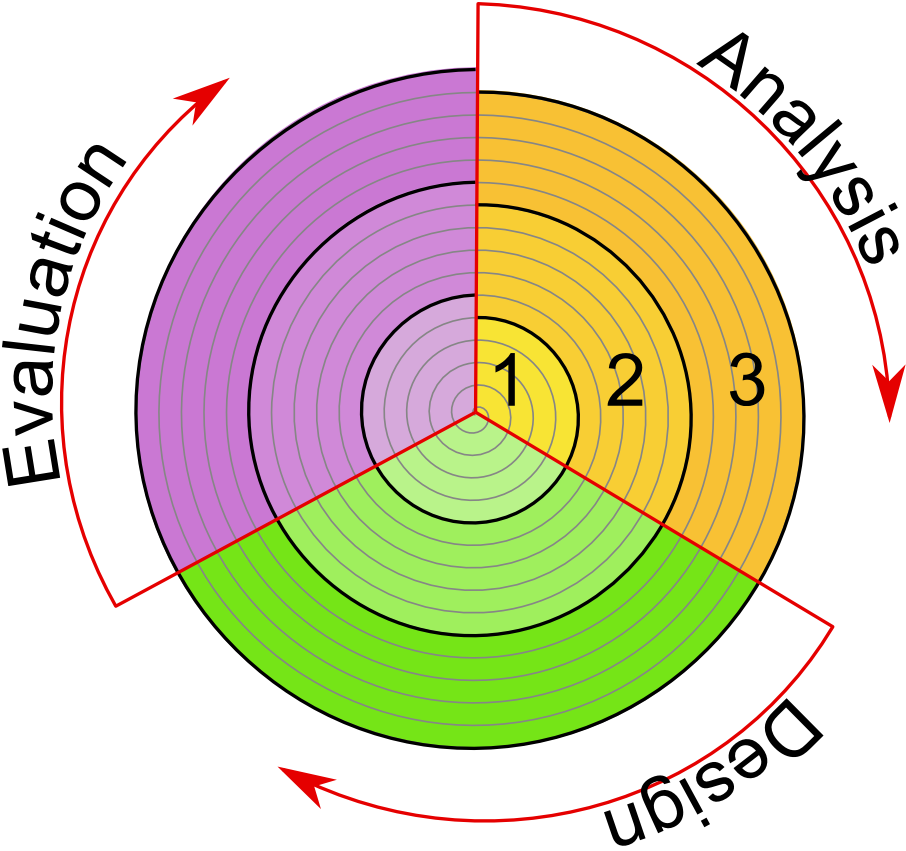
\includegraphics[width=0.5\textwidth]{espiral2.png}
\caption{ \label{intro_spiral} The user centered design process}
\end{figure}

During the analysis phase, all the information gathered from the subjects should be sorted and analyzed. Patterns and common needs should be made evident, and design decisions should be made based on these observations. It is crucial that the proposed solution respects current standards and that it integrates well with current tools. Designers should also implement the language used by final users instead of the technical terms used inside.  Proposed functionality should manifest as prototypes which may then be used for the evaluation phases. The users are engaged again in order to assess if the design is on the right track and the necessary adjustments are being made. During this process additional questions or use cases may emerge, potentially motivating the need for additional information from users. All of this information becomes input for the next iteration.

%Respect standards
%Play nice with current tools
%Language of the users
%Cite UX-book
%Be a listener
%Users hide ignorance, thy try to appear smart

\section{Objectives}

This thesis addresses the challenge of developing tools for supporting exploratory analyses with cohort data, applying the principles of visual analytics and human centered design. A model of how data and analysis tasks interact in a typical exploratory scenario is used as the foundation for the design and development of a tool to facilitate exploratory analysis of brain data. Using this model and a user-centered design process with practicing neuroscience researchers, a prototype tool called BRAVIZ is developed. To evaluate the prototype it was used in a large study, and it had a significant impact of how researchers use their data. In summary, objectives of the thesis are:

%Objectives
\begin{itemize}
\item Create a model of cohort data and visual analysis tasks that can be used to guide the design of exploratory analysis tools for cohort data.

\item Implement a prototype based on the model to validate it in the brain studies case.

\item Evaluate the prototype with a real brain study, real users and real tasks.

\end{itemize}

The research focuses particularly on multi-disciplinary teams of users. These teams generally include people with a wide variety of expertise such as radiology, imaging physics, physiology, neurology, cognitive psychology, statistical analysis, and many others. In addition, such teams are generally interested in looking at each subject's data as a whole, instead of looking at each data source independently. Interactions within and between the different specialists are considered inside the model.

%Hypotheses
The working hypothesis is that  current tools are not ideal for exploratory analysis of cohort brain data. Exploratory analysis is more efficient when only specific functionality is exposed to the user and the rest is handled automatically, without user interaction. In particular repetitive tasks and complexities in data access are barriers.

In order to assess this need it is necessary to determine several aspects and priorities of the neuroscience research community. How often is exploratory analysis done? If not often, then why? How can it be made more efficient? How can it involve more people? What are the main bottlenecks that limit exploratory analysis? This work addresses only the technological bottlenecks, but certainly other types exist, for example cultural or political. The ultimate goal of this work is to make exploratory analysis more viable, which in turn means making better use of the data and thus encourage more researchers to adopt reproducible research practices, open data, open source software, and in general, facilitate a more collaborative model for science.

%Research questions


%What are the requirements for visual exploration in cohorts?
%What are the most important tasks?
%What is the appropriate level of detail?
%How can multiple points of view be supported?
